\documentclass{sig-alternate}
\usepackage[section]{algorithm}
%\usepackage[]{algorithm2e}
\usepackage{algorithmic}
\usepackage{balance}
\usepackage{makecell}
\usepackage[usenames,dvipsnames]{color}
\usepackage[10pt]{moresize}
\usepackage[font=small,skip=0pt]{caption}
%\newenvironment{definition}{\begin{defn}\begin{em}}{\end{em}\end{defn}}
\newcommand{\inred}[1]{{\color{BrickRed}\sf\textbf{\textsc{#1}}}}
\newcommand{\card}[1]{|#1|}
\newcommand{\norm}[1]{\left\lVert#1\right\rVert}
\newcommand{\bfd}{\mathbf{d}}
\newcommand{\bfu}{\mathbf{u}}
\newcommand{\bfq}{\mathbf{q}}
\newcommand{\Z}{\mathbb{Z}}
\DeclareMathOperator*{\argmin}{arg\,min}
\DeclareMathOperator*{\argmax}{arg\,max}
\newtheorem{definition}{Definition}
\newtheorem{theorem}{Theorem}[section]
\newtheorem{thm}{Theorem}[section]
\newtheorem{lemma}[theorem]{Lemma}
\newtheorem{proposition}[theorem]{Proposition}
\newtheorem{corollary}[theorem]{Corollary}
\newtheorem{Assumption}[theorem]{Assumption}
\newtheorem{Condition}[theorem]{Condition}
\newtheorem{exe}
[thm]{Exercise}
\newtheorem{eg}[thm]{Example}
\newtheorem{conj}[thm]{Conjecture}
\newcommand{\comment}[1]{\frameit{Comment}{#1}}%
\newcommand{\note}[1]{\frameit{Note}{#1}}
\newcommand{\todo}[1]{\frameit{To-do}{#1}}
\newcommand{\inote}[1]{\inred{$<<<${#1}$>>>$}}
\newcommand{\frameit}[2]{
    \begin{center}
    {\color{BrickRed}
    \framebox[3.3in][l]{
        \begin{minipage}{3in}
        \inred{#1}: {\sf\color{Black}#2}
        \end{minipage}
    }\\
    }
    \end{center}
}

\begin{document}

\sloppy
\newcommand{\para}[1]{\par \bigskip \noindent {\bf #1.}}
\newcommand{\spara}[1]{\par \bigskip \noindent {\sc #1.}}

\newcommand{\ymatrix}[1]{\mathbf{#1}}
\newcommand{\yvector}[1]{\mathbf{#1}}
\newcommand{\ytrans}[1]{#1^{\mathsf{T}}}

\newcommand{\yset}[1]{\mathcal{#1}}

%

\title{Click-Based Content Recommendation for Semantic Stream}
%\subtitle{[Extended Abstract]
%\titlenote{A full version of this paper is available as
%\textit{Author's Guide to Preparing ACM SIG Proceedings Using
%\LaTeX$2_\epsilon$\ and BibTeX} at
%\texttt{www.acm.org/eaddress.htm}}}
%
% You need the command \numberofauthors to handle the "boxing"
% and alignment of the authors under the title, and to add
% a section for authors number 4 through n.
%
% Up to the first three authors are aligned under the title;
% use the \alignauthor commands below to handle those names
% and affiliations. Add names, affiliations, addresses for
% additional authors as the argument to \additionalauthors;
% these will be set for you without further effort on your
% part as the last section in the body of your article BEFORE
% References or any Appendices.

\numberofauthors{1}
\author{
%\alignauthor Ruiqiang Zhang\\
%\affaddr{Yahoo! Labs}\\
%\affaddr{Sunnyvale, CA, USA}\\
%\email{\normalsize \{ruiqiang\}@yahoo-inc.com}\\
}

\maketitle
\begin{abstract}

\end{abstract}

% A category with only the three required fields
%\category{H.3.m}{Information Search and Retrieval}{Miscellaneous}

%\terms{Algorithms, Experimentation}

\keywords{ }


\section{Introduction}



Developing efficient and accurate personalized recommendation systems of 
news-worthy content has been a focus of today's media industry. 
On the one hand search engines have enabled users to locate articles or 
multimedia content of any topic within a few keystrokes. On the other hand, 
users are constantly overwhelmed by the amount of information generated 
everyday, much of which is irrelevant to their personal interest. Thus directory-style news streams organized by categories are becoming increasingly popular. 

Under the latter framework, we not only need to recommend generically interesting articles, but those within a specific category, such as sports, finance, or technology, to a diverse array of users. Underneath each broad category lies more sub-categories that facilitate users to find relevant and interesting content quickly (Figure~\ref{hierarchy}).
\begin{figure}[H]
\centering
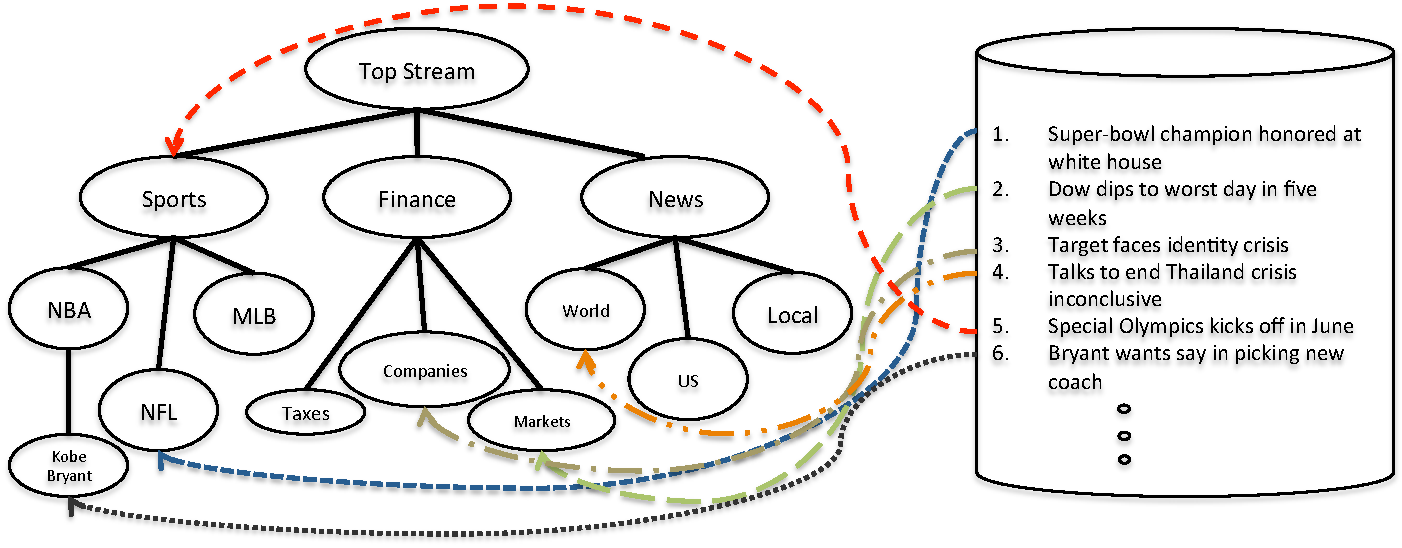
\includegraphics[scale=0.3]{Hierarchy.pdf}
\caption{Semantic Stream Hierarchy} \label{hierarchy}
\end{figure}

One obvious approach to the hierarchical stream problem is to reduce it back to the problem of a single stream, by implementing a filter for each category node on the content hierarchy. Indeed this will be an important step in the system described below. One outstanding challenge in this direction is the labeling of training examples. Given the number of streams (easily in the 100's) in question, editorial resource becomes limited. We address the problem with a combination of user click feedbacks and editorial labeling.

Even after the filter problem is solved, users frequenting different category streams can have very different sets of browsing interest. Furthermore, articles that are popular in a general stream may be less popular in a substream, and vice versa. In short, going to a lower stream category can be viewed as a probabilistic conditioning of the general user and document features distribution. Each stream therefore may require its own personalization and ranking model for optimal user experience. Scalability is again a major practical concern here. In addition, many streams have very limited user statistics to build a meaningful and robust model, which suggests that we take a holistic approach by combining streams at lower branches of the hierarchy for model training.

Justified by the above reasoning, we therefore propose a system design with essentially 2 components: a category stream filter based on linear classifier (phase 0) followed by a personalization and ranking machine. Due to runtime constraint, the latter is further subdivided into three phases, with phase 1 selecting among hundreds of thousands of articles only the top 200 candidates according to stream relevance and user preferences, using a simple linear model with only positive weights (negative pruning). The features consist of entity scores within the user and document profile, the popularity score of the article, measured in terms of discounted CTR, and finally the freshness of the content. Phase 2 then performs re-ranking of those 200 articles using the more sophisticated Gradient Boosted Decision Tree (GBDT) model. Finally phase 3 takes into account pairwise similarity of those 200 articles and slightly reorganize them to achieve better diversification. Altogether, the three phases yield an efficient approximate solution to the optimal ranking problem; an exact solution is clearly too expensive for any reasonably sized content/user pools.

Phase 0 can arguably be combined with phase 1, since both have linear forms. This is the spirit of model \eqref{original SRQ}. In practice, however, we find the latency unacceptable when applying the algorithm during serving time, since document profiles can have significantly more features than users. Instead, phase 0 takes away some of the burden in \eqref{original SRQ} by computing the document-only component scores during content ingestion time, and a simplified phase 1 model \eqref{practical SRQ} is adopted for fast document retrieval.

We demonstrate order of magnitude improvement in precision-recall of the linear classifier over tfidf approach. Compared with decision rule based approach, the classifier significantly increases recall while keeping precision the same or better. For phase 1 personalized stream-specific linear ranking, we measure the performance in terms of click/skip ROC curves and show an increase in Area Under the Curve (AUC) of 3-4\% under model \eqref{practical SRQ}  over the stream-independent model. The exact metric definitions are reviewed in Section~\ref{evaluation metrics}.

To summarize, we design a highly efficient, scalable stream content recommendation system that optimizes user experience measured in terms of CTR, by seeking a balance among the following five desirable attributes: relevance (to the individual stream), popularity, freshness, personalization, and diversity. 


%One of the earliest prototypes of personalized ranking system is based on a 
%simple linear matching model of user interest profile and document topic 
%profile. This crude approach has proved effective in promoting highly relevant 
%articles, videos or slideshows to each individual user, even when we have only 
%accumulated partial information about the user. Unfortunately there are 
%several drawbacks to this simple model. First the dot product between the user 
%profile and document profile is not necessarily a natural one, since both 
%profiles are calibrated separately, with no natural complementary ``units" 
%relating the two. An immediate remedy is to learn a non-Euclidean inner 
%product with suitable objective functions such as click through rate or 
%dwell-time. Second, while the linear model presents a ranking order of 
%documents based on user's implicit or declared interest, it nonetheless does 
%not take into account generic information such as user's age, gender, time of 
%the day, day of the week, etc, which could be crucial to users' preference 
%among the top documents presented. These are the actual content that the user 
%sees, which clearly requires more careful optimization than the entire content 
%pool. 
%
%A second challenge goes back to the initial selection of content itself. While 
%general news streams certainly occupy the central stage in terms of breadth of 
%user coverage, there tends to be less depth and personalization opportunity 
%involved in their content. Users who are interested in a specific category of 
%news such as sports or finance, or even narrower ones like American football, 
%are naturally interested in dedicated streams just for those topics. Indeed 
%this is how one accumulates domain-specific expertise as opposed to common 
%knowledge. Thus we are interested in constructing appropriate filters 
%conforming to prescribed semantic topics. 
%
%In this paper we will address the second problem with a carefully designed 
%linear classifier framework based on a combination of user click feedback and 
%editorial label. We compare the performance of the classifier approach with 
%the baseline TFIDF (token-frequency inverse-document-frequency) approach. 
%


\section{Related Work}

\section{System Design}

\subsection{Motivations}
Designing an actionable system for thousands of article streams with millions of content to present is a highly nontrivial task that requires both  latency consideration and machine learning insight. The latter can further be divided into several categories of objectives, such as relevance, freshness, personalization, segmented popularity, etc. In order to build an agile and well-focused pipeline, it is imperative to modularize the effort into different phases. Thus we devote a document classifier phase (phase 0) to optimize for relevance, an pre-screening stream-specific linear matching phase (phase 1) to optimize for serving-time latency, followed by a more powerful ranking algorithm (phase 2); both phase 1 and phase 2 take into account personalization and popularity. Finally we want to ensure that similar articles stay far from one another, a task that requires pairwise comparison operations, hence must be addressed separately at the end (phase 3). In general, Having a multi-phase system can be a challenge in bucket tests or even offline optimization. Fortunately, due to their conceptual independence, we argue that it is relatively harmless to optimize them in parallel. 


\subsection{Phase 0: Document Classifier}

In the past the classification task for semantic streams was trivialized to the manual selection of logical filter criteria based on a basket of pre-engineered in-house topical features, or extracted wiki entities, along with their aboutness scores. This approach has the obvious drawback that not all classification criteria can be compactly summarized by a handful (certainly fewer than 100) of logical conjunctives and disjunctives. In fact, since many of the pre-constructed features were not motivated by the stream classification tasks that we are dealing with, chances are they might be completely irrelevant or inaccurate in capturing the essence of the stream definitions. Thus we propose to learn the filter directly from the textual bodies of the articles themselves. In theory at least, this would learn a model that's at least as accurate as the ones obtained from the aforementioned logical patchwork. In reality, however, since logical connectives require higher order non-linear features to exactly replicate, the cost of training an identical model based on token features could be high. As we will show in the experimental results section below, however, even with simple unigram model, the precision-recall of a freshly trained model well outperforms the ones based on logical filters constructed by domain experts. Even for a stream as clearly defined as NFL, brute force human filter construction reveals that there are many edge cases (e.g. when both college football players and NFL players appear in the article, or when Super Bowl is mentioned along with other local news) that must be handled with specialized rules, which together can easily go into hundreds of terminal decision nodes. 

  As a baseline, we also consider the term-frequency inverse-document-frequency (TFIDF) approach, whereby a centroid vector is constructed for each stream based on the number of appearances of each token stem in the stream, weighted by inverse of the logarithm of the total number of documents in which it appears:
\begin{align*}
C^{\mathcal{S}}_{t_i} =\card{\{k \in [\dim \mathcal{S}]: \mathcal{S}_k = t_i  \}} / \log \card{\{d \in \mathcal{D}: t_i \in d\}}.
\end{align*}
Here $\mathcal{S}$ stands for the concatenated vector of all tokens from the training set articles in the stream, $C^{\mathcal{S}}$ stands for the centroid vector for the stream represented by $\mathcal{S}$, and $\mathcal{D}$ is the universal set of all documents.

  TFIDF is appealing in its dependency mainly on the positive examples; one could think of the entire universe of content pool as representing the negative examples, however the accuracy of the negative labels in this sense is not strictly enforced. More sophisticated variants of TFIDF exist such as instead of a single centroid vector, using a generative model to learn a set of vectors and compute distance of a new candidate document to each of those vectors as a high-dimensional similarity metric. However we feel that the potential gain on top of a simple linear classifier approach does not quite justify the increased model complexity. 

  Finally we also mention that there are several one-class classification strategies, such as those based on density estimation, clustering, and kernel SVM, but again the increased model complexity can be a strong hurdle to execution, and the fact that negative examples are not leveraged at all makes them less than ideal.

\subsubsection{Data Collection}
  Independent of the model choice, it is important for us to choose a set of positive examples and negative examples as our initial training set. Due to the large quantity of articles and variety of topics in each stream, as well as the sheer number of streams we are dealing with (ultimately in the thousands), complete reliance on editorial judgment is clearly infeasible. Instead we opt for the following heuristic approach of labeling the articles as to their appropriateness for a particular stream. 

  For the streams already in production, we have a natural signal for stream appropriateness label, namely the user click feedback. Thus we label all the articles surfaced on the stream, that received at least 5 unique user clicks, as the positive examples. The assumption is that users who visit a particular stream are most likely interested in content pertaining to the stream definition. Having multiple users interested in a document is a good sign that the article is not just interesting from a general point of view, but is also relevant to the stream. Thus we expect high precision of such labeled set but low recall, as many articles never see the light of day due to low popularity score, which is part of the production ranking criterion, and we are also potentially missing out on the articles that the production filter fails to capture. 
   
   Because of the low-recall concern with the above approach, we need to be somewhat careful in selecting the negative examples. In general we want to avoid false negatives at the expense of true negatives, since there are typically many more negative examples than positive examples. The most scalable solution turns out to be including all articles that do not pass the production filter. This is clearly the right thing to do since weakly positive examples (ones that didn't receive enough user clicks) could nonetheless be highly relevant. 

  For streams not yet launched, clearly domain expertise is required to initialize the classifier. Fortunately we have a variety of well-polished features, such as topical categories, tagged named entity, etc, that can be combined through logical connectives to yield an approximate profile for the stream. Once that gets launched and starts receiving user clicks, subsequent batch active-learning cycles will be able to learn the model and fine-tune it to suit the user interests. There is always the risk of flooding a specialized stream with generally popular topics (such as Kim Kardashan in the Sports stream or MH370 in the Finance stream), if we base our model evolution solely on user responses. Thus we require periodic editorially judgment to be injected into the positive and negative training set as well, in a balanced manner to account for the relative paucity of editorial resource compared to user signals.

  To be sure, we do not expect close to perfect precision or recall from the simple classifier approach outlined here. In fact the training data itself is highly susceptible to noise, especially those gathered according to the user click heuristics. 

\subsubsection{Feature Selection}
We compared the relative performance of 6 distinct families of features, listed below:
\begin{itemize}
\item title and body token stems and frequency counts
\item in-house topic categories and aboutness scores
\item wiki entities and aboutness scores
\item named entities and aboutness scores
\item editorial tags as binary features
\item publisher ids as binary features
\end{itemize}

After extensive experimental comparison, we found that while the topic category and publisher id together achieve high performance on testing, it could be that we are simply relearning the production model, which depends almost exclusively on these features. On the other hand, token stem frequencies alone perform remarkably well on validation set compared to all other combination of features from the above list. The performance on testing is markedly worse than the former, but againt this could be due to noisy labels. Since our ultimate goal is to learn the validated labels, and that tokens are primitive features, unadulterated with intermediate processing, we choose them for all streams.


\subsubsection{Model Selection}
Equipped with labeled positive and negative examples and their respective unigram token features, we are in the standard setting of a binary classification task. The combined training and testing set size is about 50k for each top level stream (such as Finance and Sports) and 10k for secondary stream, with NFL being the only example considered at this level. The split between training and testing set is 70\% to 30\%. The ratio of negative to positive examples is typically in the range of 3 to 5 for top streams, but can get much wider for lower level streams. During training we artificially inflate the positive examples to ensure equal weighting. 

 In addition, we prepared a validation set of about 3000 articles for the top level streams for editorial labels. These will not only form a validation golden set for the initial model trainin, but will be recycled for future model updating with appropriate weight that decays with time. 

Three model performance metrics are thus considered (training, testing, and validation), each of which is based on precision recall AUC. For secondary streams such as NFL, we found that a one against all (OAA) approach results in significantly worse metrics than the top stream. This is most likely due to the severe imbalance between positive and negative examples. Fortunately since NFL belongs to Sports as a substream, we could filter out majority of the negative examples that do not pass the Sports filter. This seems a generally applicable strategy despite the fact that there are occasional articles that belong to the lower stream but not to the top. 

  To continue with the Sports-NFL example, we currently use the production Sports filter as the pre-screening device for NFL articles. In the future, when the Sports filter is replaced by the trained classifier model, we are afforded more flexibility in adjusting the pre-screening strength. How to select the pre-secreening parent classifier threshold ties intimately with the ultimate precision-recall requirement. 

Finally to determine the exact classifier form, we found that the performances of logistic loss and hinge loss (SVM) are comparable. However since our preferred training tool, Vowpal Wabbit with L-BFGS optimizer, supports logistic regression far better than SVM (as hinge loss is non-differentiable), we settled upon logistic regression. Some further exploration reveals that a ridge regularization parameter of $10$ works well for all three streams tested, and on both testing and validation sets. 

\subsection{Phase 1: Twisted Dot Product}

As alluded to before, the classifier instrumented at Phase 0 is not perfect, in particular we do not anticipate 100\% precision. Thus the burden is on subsequent phases to remove any embarassing candidate article for each stream. The Stream Relevance Query (SRQ) proposed at Phase 1 provides the second line of defense against the irrelevant articles. Furthermore it can be viewed as an optimization step for the more serious ranking done at Phase 2. 

In a nutshell, SRQ is a stream-enhanced version of the following generic model applied to the entire content pool:
\begin{align*}
\rm{score}_1 =  (\alpha_0  \rm{gmp} + \alpha_1  \langle \bfu,\bfd\rangle ) e^{-\beta \Delta T}.
\end{align*}
Here $\bfu$ denotes the user profile vector, consisting of the sparse polarity scores of all the topical categories and wiki entities, in a sparse format, since a typical user exhibits above average interest in only a couple dozens out of hundreds of thousands of entities. The vector $\bfd$ consists of document features, expressed in the units of aboutness score. $\rm{gmp}$ is a popularity score determined essentially by CTR of the article. $\Delta T$ is the time since publishing of the article, which captures the freshness of the article. Thus the exponential factor promotes more recent articles. The weights $\alpha_0, \alpha_1$, and $\beta$ are either trained offline or tuned with split online buckets. 

The originally proposed SRQ recipe takes the following form:
\begin{align} \label{original SRQ}
\rm{score}_{\rm{SRQ}} = (\alpha_0 \rm{gmp} + \alpha_1 \bfq_0 \cdot \bfd + \alpha_2 \bfq_1 \circ \bfu \cdot \bfd ) e^{-\beta \Delta T}.
\end{align}
Thus we replace the original dot product $\alpha_1 \bfu \cdot \bfd$ with a twisted (triple) dot product $\alpha_1 \bfq_0 \cdot \bfd + \alpha_2 \bfq_1 \circ \bfu \cdot \bfd$. Alternatively, one can think of the the twisted product as a modification to the user profile $\bfu \mapsto \bfu' := \alpha_1 \bfq_0 + \alpha_2 \bfq_1 \circ \bfu$. This admits tremendous flexibility in relevance-biased personalization; each user thus can put on many different ``faces" when interacting with the different streams.

One caveat to the above enhancement is that the new stream-specific user profile $\bfu'$ can now have hundreds of thousands of nonzero entries, making it non-sparse. On the other hand, the Homerun phase 1 relies heavily on the sparsity of the user feature vector to optimize for latency, essentially by dropping candidate articles that do not match the user vector on any entity (hence results in $0$ dot product), unless $\bfu$ is too sparse, in which case $\rm{gmp}$ dominates and the top ranked articles by popularity get selected. Having a dense $\bfu'$ makes it significantly harder to implement such optimization heuristics. So we instead consider the following practical SRQ model:

\begin{align} \label{practical SRQ}
\rm{score}_{\rm{pSRQ}} = (\alpha_0  \rm{gmp} + \alpha_1 \bfq \circ \bfu \cdot \bfd) e^{-\beta \Delta T}.
\end{align}
The main difference is the removal of the old-fashioned dot-product term. One could argue non-rigorously, that the Phase 0 filter is essentially performing the same job as the zeroth order term $\alpha_1 \bfq_0 \cdot \bfd$ in the original SRQ model. 

Other variations that do not completely lose the document-only signals include the following indicator model:

\begin{align*}
\rm{score}_{\rm{iSRQ}} = (\alpha_0 \rm{gmp} + \alpha_1 \bfq_0 \circ \chi(\bfu) \cdot \bfd + \alpha_2 \bfq_1 \circ \bfu \cdot \bfd ) e^{-\beta \Delta T},
\end{align*}
where $\chi(\bfu) = (1_{u_1 > 0} ,\ldots, 1_{u_m > 0})$ is the component-wise indicator vector for $\bfu$. Under $\rm{iSRQ}$, the user vector $\bfu$ gets transformed into an equally sparse tilted $\bfu' = \alpha_1 \bfq_0 \circ \chi(\bfu) + \alpha_2 \bfq_1 \circ \bfu$ that closely resembles the original $\rm{SRQ}$, $\bfu'$.

Regardless of the actual scoring formula used, the output of Phase 1 ranking is a set of around 200 articles, to be ranked further by Phase 2 GBDT machinery. This reduction from thousands of articles facilitates highly sophisticated algorithms to be applied for accurate personalized ranking.

\subsection{Phase 2: Boosted Ranking}
\input phase2
\subsection{Phase 3: Diversity}

All the previous phases in the stream content recommendation pipeline only consider the candidacy of individual articles independent of one another. If the entire stream only recommends a single article, this approach clearly achieves its objective well, namely outputs the top article in the final ranking at the end of Phase 2. However the actual stream user experience can be viewed as a high-dimensional optimization problem, in which the whole might not be equal to the sum of the parts. In other words, there could be negative correlations between two articles at distinct positions. The most obvious example is given by similar articles that are placed next to each other. User experience clearly drops due to redundancy; an opportunity to present slightly less compelling content in one of the positions is also lost. In practice, with the current production algorithm, we have seen even 3 or 4 articles with closely related content being ranked near one another, since they tend to have very similar phase 2 scores. 

We propose two strategies to overcome the ``curse of similarity".  The first strategy seeks an optimal linear combination of Phase 2 score and a dissimilarity score with a carefully chosen set of other articles. Two choices of the dissimilarity sets are considered here (code-named v1 and v2 respectively). The second strategy is a greedy approach that keeps as many Phase 2 top-ranked articles as possible that maintain pairwise similarity score below some threshold (algorithm v3).

\subsubsection{Diversity Version 1}
First we fix a few notations/definitions: 
\begin{itemize}
\item The meaning of document profile $\bfd$ here differs slightly from the previous phases: the underlying building blocks are topic/wiki entities aboutness scores, just as in Phase 1. However we re-weight the scores by a relative inverse document frequency $1/ \log \card{\{d \in \mathcal{D}_{200}: t_i \in d\}}$, where $D_{200}$ is the 200 articles received from Phase 2 only, instead of the entire content pool of size 1m. The purpose of this polarity adjustment is to ensure that streams with highly homogeneous content, such as NFL, have similar feature distribution, in terms of pairwsie similarity distance, as the ones that are more diverse, such as the Finance stream. This ensures that a unified model can be applied to all streams, regardless of level of specialization.
\item the similarity score between two articles $\bfd$ and $\bfd'$ is simply the cosine distance ($\ell^2$ normalized inner product): $\rm{sim}(\bfd,\bfd') = \langle\bfd,\bfd'\rangle/(\norm{\bfd}_2 \norm{\bfd'}_2)$.
\item $\bfd_i$ denotes the article with $i$th highest phase 2 score, whereas $\bfd'_i$ denotes the articles with $i$th highest phase 3 score after the diversity algorithm is applied.
\item The phase 2 scores $\rm{score}_{p2}$ are normalized via an affine transformation so that the top scoring article and bottom scoring articles receive scores of $1$ and $0$ respectively.
\end{itemize}

Algorithm v1 tries to learn a single parameter $\lambda \in [0,1]$ in the following ranking score formula, based on both phase 2 scores and pairwise similarity, defined inductively from top to bottom of the stream.

\begin{align}
\bfd'_1 =& \argmax_{\bfd' \in \mathcal{D}_{200}} \rm{score}_{p2} (\bfd') \label{v1 init}\\
\bfd'_k =& \argmax_{\bfd' \notin \{\bfd'_1, \ldots \bfd'_{k-1}\}} \lambda \times \rm{score}_{p2} (\bfd') \nonumber\\
&- (1- \lambda)\max_{\bfd: \rm{score}_{p2}(\bfd) > \rm{score}_{p2}(\bfd')} \rm{sim}(\bfd_i, \bfd'). \label{v1 mid}
\end{align}

The v1 scores associated with each document are thus the maximum values achieved in the formulae above, which takes the following simple form:
\begin{align}
\rm{score}_{v1}(\bfd_k) = \lambda \rm{score}_{p2}(\bfd_k) - (1-\lambda) \max_{i< k} \rm{sim}(\bfd_i,\bfd_k) \label{v1 score}.
\end{align}
 In particular, the top phase 3 document $\bfd'_1$ coincides with the top phase 2 document $\bfd_1$ and always receives a phase 3 score of $1$. Observe that the set of ``other documents" we compare the $k$th candidate document $\bfd'_k$ to consists of articles with higher phases 2 scores than $\bfd'_k$. Note also that the inductive step \eqref{v1 mid} does not depend on the ranking results of the previous step; one can compute v1 scores according to formula~\ref{v1 score}, and rank the articles based on those. This suggests a natural $O(n^2)$ algorithm, where $n$ is the number of articles (typically around $200$).

In online experiments, we segment the $\lambda$ values into 5 bins: $\{0.65,0.70,0.75,0.80,0.85\}$ based on offline observations. We then compare key metrics for each of the 5 sub-buckets and choose the strongest performer. In general, smaller $\lambda$ corresponds to more diverse set of top documents, obviously at the expense of demoting highly relevant and personalized articles towards the bottom. As illustrated in Appendix~\ref{appendix diversity}, v1 often does a poor job at separating similar articles beyond the first few in the stream, because the linear combination of phase 2 score and diversity score simply does not ensure any local separation.

 As an extreme example, consider two identical articles $\bfd_\alpha$ and $\bfd_\beta$ in the stream,  that in practice would not occur due to the de-duplication procedure in earlier phases. Clearly they have the same phase 2 score, $\rm{score}_{p2}(\bfd_\alpha) = \rm{score}_{p2}(\bfd_\beta)$. If their diversity scores also happen to be close relative to other documents, then they will be ranked next to each other. To guarantee the latter, that is, $\max_{i \in [k-1]} \rm{sim}(\bfd_i,\bfd_\alpha) \approx \max_{i \in [k]} \rm{sim}(\bfd_i,\bfd_\beta)$, one simply requires that $\rm{sim}(\bfd_k,\bfd_\beta) < \max_{i \in [k-1]} \rm{sim}(\bfd_i \bfd_\beta)$, which is not unlikely provided $\bfd_\alpha \notin \{\bfd_i: i \in [k]\}$. 


%
%\subsubsection{Diversity Version 2}
%The algorithm v2, also based on the idea of linearly combining phase 2 score and diversity score, takes the same initializing form as \eqref{v1 init} and diverges subtly from v1 in the inductive step \eqref{v1 mid}:
%\begin{align}
%\bfd'_k &= \argmax_{\bfd' \notin \{\bfd'_1, \ldots \bfd'_{k-1}\}} \lambda \times \rm{score}_{p2} (\bfd') - (1- \lambda)\max_{i\in [k-1]} \rm{sim}(\bfd'_i, \bfd'). \label{v2 mid}
%\end{align}
%Thus the only difference is to replace $\bfd_i$ in the final similarity function by $\bfd'_i$, that is, the phase 2 relative ranking is no longer used (however, the phase 2 scores are clearly still needed).
%
%The use of phase 3 ranking directly in the inductive step avoids the duplicate article pathology for v1. However by the nature of linear combination itself, two identical articles can still be ranked close to one another, if the ``right" $\lambda$ is chosen. An additional complication is run-time complexity. Following the inductive recipe \eqref{v2 mid} directly requires $O(n^3)$ number of comparison. Fortunately there is a trick (due to Qili Chen) to reduce it to $O(n^2)$, provided we get an additional $O(n)$ space storage on top of the $O(n^2)$ required for storing the pairwise similarity distance. 
%
%\begin{algorithm}[H]
%\caption{
%$O(n^2)$ algorithm v2
%}\label{alg:nsq_v2}
%\begin{algorithmic}[1]
%\REQUIRE 
%1) Pairwise similarity table $\rm{sim}(\bfd_i,\bfd_j)$, $1 \le i < j \le n$;
%
%2) Phase 2 scores $\rm{score}_{p2}(\bfd_i)$, $1 \le i \le n$;
%
%3) $\lambda$.
%\ENSURE
%Phase 3 rankings $\{\bfd'_i: 1 \le i \le n\}$ according to v2 formula \eqref{v2 mid}. 
%\STATE Initialize maximal similarity hashtable $M$\;
%\STATE Set $\bfd'_1  \longleftarrow \bfd_1$\;
%\FOR{$i = 2, \ldots, n$}
%\FOR{$\bfd \notin \{\bfd'_1, \ldots, \bfd'_{i-1}\}$}
%\IF{$i==2$}
%\STATE $M(\bfd) \longleftarrow \bfd'_1$\;
%\ELSE 
%	\IF{$\rm{sim}(\bfd,M(\bfd)) < \rm{sim}(\bfd,\bfd'_{i-1})$}
%		\STATE $M(\bfd) \longleftarrow \bfd'_{i-1}$\;
%	\ENDIF
%\ENDIF
%\STATE $\rm{score}_i(\bfd) \longleftarrow \lambda \rm{score}_{p2} (\bfd)- (1-\lambda) \rm{sim}(\bfd,M(\bfd))$\;
%\ENDFOR
%\STATE $\bfd'_i \longleftarrow \argmax\{\rm{score}_i(\bfd): \bfd \notin \{\bfd'_1, \ldots, \bfd'_{i-1}\}\}$\;
%\ENDFOR
%
%\RETURN $\bfd'_i$, $1 \le i \le n$.
%\end{algorithmic}
%\end{algorithm}


\subsubsection{Diversity Version 3}
Both version 1 and 2 above suffer in the following two areas:
\begin{itemize}
\item There is no theoretical guarantee that similar articles do not cluster in positions;
\item Everything being equal, the phase 2 ranking is not well-respected.
\end{itemize}
The second issue above renders these algorithms in principle not a strictly improvement over no diversity at all. We therefore propose a third alternative, which is closely related to clustering. Briefly, we construct a cheap collection of article clusters and choose the top one (according to phase 2 score) within each to populate the first batch of articles, and inductively populate the later batches. Instead of constructing the clusters all in advance, the algorithm ``discovers" elements within each cluster from top to bottom, one batch at a time. A $\lambda$ parameter is set as an upper bound for the pairwise similarity distance among articles within each batch. We do not guarantee diversity between batches. 

Algorithm v3 thus solves the following constrained optimization problem:
\begin{align}
&\min_{k \in \Z_+, \sigma \in S_n } k \label{v3 optimization}\\
&s.t. \; \exists  \:0 =b_0 < b_1 < \ldots < b_k = n, \nonumber\\
&\rm{sim}(\bfd_{\sigma(u)},\bfd_{\sigma(v)}) \le \lambda ,\; \sigma(u) \le \sigma(v), \; \sigma(b_{i-1}) \le \sigma(b_i) \nonumber\\
&\forall \: b_{i-1} < u < v \le b_i, \: i \in [k] \nonumber
\end{align}

The condition $\sigma(b_{i-1}) < \sigma(b_i)$ ensures that the top article from phase 2 is again ranked the highest under phase 3. In the algorithm below, $B_c$ stands for the current batch, and $B_r$ stands for the union of the remaining batches. 

\begin{algorithm}[H]
\caption{
Clustering based algorithm v3
}\label{alg:v3}
\begin{algorithmic}[1]
\REQUIRE 
1) document feature vectors $\bfd_i$, $1 \le i \le n$;

2) Phase 2 scores $\rm{score}_{p2}(\bfd_i)$, $1 \le i \le n$;

3) $\lambda$.
\ENSURE
Phase 3 rankings $\{\bfd'_i: 1 \le i \le n\}$ satisfying \eqref{v3 optimization}. 

\STATE Initialize $B_r \longleftarrow (\bfd_1, \ldots, \bfd_n)$\;
\WHILE{$B_r$ not empty}
\STATE Initialize $B_c \longleftarrow ()$\;
\FOR{$\bfd \in B_r$}
\STATE Demote $\longleftarrow$ False\;
\FOR{$\bfd' \in B_c$}
\IF{$\rm{sim}(\bfd,\bfd') > \lambda$}
\STATE Demote $\longleftarrow$ True\;
\ENDIF
\ENDFOR
\IF{Demote == False}
\STATE Append $\bfd$ to $B_c$\;
\ENDIF
\ENDFOR
\STATE Remove all $\bfd \in B_c$ from $B_r$\;
\STATE Output $B_c$ as the next batch.
\ENDWHILE
\end{algorithmic}
\end{algorithm}
Depending on the size of the final batches, the run time complexity of Algorithm~\ref{alg:v3} lies somewhere between $\Omega(n)$ and $O(n^2)$. For instance, if all batches are of size $1$, or if there is a single batch of size $n$, then $\binom{n}{2}$ comparisons are needed. But if say all batches are of size $\sqrt{n}$, then a heuristic calculation, based on the assumption that the admissible articles within each batch are spaced evenly apart from one another in the original phase 2 order, shows that if there are $k$ batches with average batch size $\alpha = n/k$, then the total number of comparisons needed would be 
\begin{align*}
\frac{k(k+1) \alpha (\alpha + 1)}{4}.
\end{align*}

Thus the best \emph{average} run-time is $n^2/4$, attained when $k = \alpha =n^{1/2}$. In theory, however, the best run-time can be much lower, since one can imagine elements within each batch excluding the top one gravitate towards the bottom of the phase 2 rankings. Another way to speed up the algorithm is by introducing a window parameter $w$ that caps the size of each batch. In that case the run time is bounded by $O(w n)$.



\section{Experiment Results}
\subsection{Evaluation Metrics} \label{evaluation metrics}
 Recall the following definition of precision recall curve. Given a test data set of size $n$, each with $m$ features, $\{(f_{ij}, p_i)\}_{i \in [n], j \in [m]}$, a binary classifier (such as SVM, logistic regression, gbdt, etc) typically outputs a score for each record $p((f_{i1}, \ldots, f_{im}))$.  The records are classified as positive or negative based on whether the score exceeds a fixed threshold $\lambda$ or not. 
\begin{definition}
Given a sequence of score-label pairs $(s_i,\ell_i)$, $1 \le i \le n$, sorted by first component then second, such that $s_i \le s_j$ for $i< j$, and $\ell_i \in \{-1,+1\}$, the Precision-Recall (PR) curve is the linear interpolation of the set of points $(r_i,p_i)$, with flat extrapolation from the leftmost point to the $y$-axis, where $p_i = \frac{\rm{TP}_i}{\rm{TP}_i + \rm{FP}_i}$ is the precision at position $i$, and $r_i =\frac{\rm{TP}_i}{\rm{TP}_i + \rm{FN}_i}$ is the recall at position $i$. Here we define
\begin{itemize}
\item $\rm{TP}_i := |\{j \le i: \ell_j =+1\}|$, the number of true labels above position $i$ (true positives),
\item $\rm{FP}_i := |\{j \le i: \ell_j =-1\}|$, the number of false labels above position $i$(false positives),
\item $\rm{FN}_i := |\{j > i: \ell_j = +1\}|$, the number of true labels below position $i$(false negatives).
\end{itemize}
\end{definition}

\begin{definition}
The Receiver Operating Characteristic (ROC) curve is defined similarly, replacing $(r_i,p_i)$ with $(f_i, t_i)$, where $f_i = \frac{\rm{FP}_i}{\rm{FP}_i + \rm{TN}_i}$ is the false positive rate at position $i$ and $t_i = \frac{\rm{TP}_i}{\rm{TP}_i + \rm{FN}_i}$ is the true positive rate. 
\end{definition}

\begin{definition}
The Area Under Curve (AUC) can be defined for either Precision-Recall curve or the ROC curve as above. If we parametrize the curve as the graph of a function $\gamma:[0,1] \to [0,1]$, the AUC is defined by
\begin{align*}
\rm{AUC} = \int_0^1 \gamma(t) dt.
\end{align*}
Note that the x-coordinates of both curves attains the maximum value of $1$, since at position $i = n$, $\rm{TN}_i = \rm{FN}_i = 0$ by definition. It is possible in theory that the x-coordinates to hit $0$, precisely when the top ranked article has a negative label. However in practical situations there is always a gap between the left most point and the y-axis, which can be addressed with any reasonable extrapolation scheme. Here we choose flat extrapolation to facilitate probabilistic calculations.

Since the curves are piecewise linear, given by linear interpolation of a finite set of $n$ points, the integral can be easily and exactly computed using the Trapezoid rule.
\end{definition}

For phase 0 stream filter, we use precision-recall AUC as the principle measure of performance. The labels are generated using either heuristic methodology based on production filter in combination with unique user click statistics, or editorial judgment. The latter data is sparse but has high fidelity. AUC of $1$ corresponds to the perfect situation where all the positively labeled articles are ranked higher than the negatively labeled ones. This does not mean that a threshold is not necessary, but only that a perfect threshold is feasible, and that for any threshold level, the total number of misclassifications is optimal (minimal) among all rankings. 

For phase 1 and 2, we use primarily AUC under the ROC curve, based on the user click feedback. Thus a clicked article $d$ by a user $u$ is considered a positive example, whereas the rest are negative examples. This is an appropriate metric here because the end goal here is ranking. AUC for ROC can be seen as a specialization of a family of permutation statistics, with notable examples such as Kendall's tau, that measures the number of pairs of records whose relative order is reversed compared to the true ranking. It is also conveniently agnostic to the ratio between the numbers of positive and negative labels. 



ROC curve is always monotone non-decreasing, which is easily seen by rewriting $t_i = \frac{1}{1 + \rm{FN}_i / \rm{TP}_i}$ and $f_i = \frac{1}{1 + \rm{TN}_i / \rm{FP}_i}$, and noticing the subfractions are both monotone in $i$. The PR curve however can be highly non-montone in general, since the quantity $\rm{FP}_i / \rm{TP}_i$ has no monotonicity in general. An easy example is given by $n-1$ positively labeled data and a single negatively labeled one: in this case the curve starts off with $p_i =1$ until the index reaches the negatively labeled datum, at which point the curve drops to $\frac{i-1}{i}$, which however is an increasing function in $i$. In a sense, the more monotone the PR curve, the better it is from predicting completely randomly.


It is important also to note that while the AUC for ROC curve always has a mean of $0.5$ under uniform ranking, easily proved using the equivalence with Mann-Whitney-Wilcoxon statistics, provided there is at least one positive example and one negative example,  the AUC for the PR curve has a uniform baseline distribution that depends on the exact ratio between positive and negative examples. Again with the example of one negatively labeled datum, where the predicted rank of the negative example is uniformly random, then using flat extrapolation to the left, the expected AUC for PR curve is given by 
\begin{align*}
\frac{1}{n} \sum_{k=1}^n [\frac{k}{n} + \sum_{i=k+1}^n \frac{i-1}{in}] = 1 + o(1).
\end{align*}
In general it's easy to show (by considering pointwise average) that the average AUC is given by $P/n$, where $P$ is the total number of positively labeled examples. This is especially important for the stream filter evaluation, since there tends to be many more negative examples than positive ones. 

Finally to measure performance of phase 3 diversity algorithm, we introduce two additional metrics. The goal is to ensure maximal diversity among the top $k$ articles in the final ranking, while preserving the ranking from phase 2 as much as possible. The first metric thus measures the diversity directly, using the geometric interpretation of determinants as the volume of $k$-dimensional parallelopiped in an $m$-dimensional Euclidean positive orthant. Here $m$ is the number of features used in the diversity algorithm, namely topic categories and wiki entities.
\begin{definition}
Given a set of ranked documents $d_i$,$ 1 \le i \le n$, each with $m$ features $\mathbf{f}_i = (f_{i1}, \ldots, f_{im})$,  we can define the top $k$ Gram-determinantal diversity to be 
\begin{align*}
d_k = \det (\langle \mathbf{f}_i , \mathbf{f}_j \rangle)_{1\le i,j \le k}
\end{align*}
The Determinantal Diversity (DD) curve is given by linear interpolation of the points $(k,d_k)$, $1 \le k \le n$. We can define similarly the AUC associated with the DD curve as before, with the technical caveat that the curve now span $[1,n]$ on the horizontal scale.
\end{definition}
 
To measure the amount of scrambling on phase 2 ranking due to phase 3 diversification, we use curves derived from two standards metrics: top $k$ Kendall's tau and top $k$ Mean Reciprocal Rank (MRR). To avoid unnecessary confusion, we will not look at AUC of these curves.

Kendall's tau can be seen as a generalization of AUC for ROC curve, where the set of labels is extended from a two-element set $\{-1,1\}$ to a set of $n$ elements, namely the rankings of all the objects. Formally we have
\begin{definition}
Given a predicted ranking sequence $\sigma(1), \ldots, \sigma(n)$, where $1,\ldots, n$ is the true ranking of the $n$ objects, the Kendall's tau of the prediction is given by
\begin{align*}
\rm{KT}(\sigma) = \card{\{ (i,j): 1 \le i< j \le n, \sigma(i) > \sigma(j) \}} / \binom{n}{2}.
\end{align*}
 Thus $\rm{KT}(\sigma)$ measures the number of ``pairwise disarrays". Under the normalization by $\binom{n}{2} = \frac{n(n-1)}{2}$, if $\sigma(i) = n-i+1$, we get the opposite ranking, with a KT score of exactly $1$.
\end{definition}

%MRR is another standard metric in ranking literature. It penalizes mis-ranking for higher ranked articles more than that for lower ranked articles, which makes sense in the current semantic stream context.
%\begin{definition}
%Given a ranking of $n$ objects $\sigma(1),\ldots, \sigma(n)$, the top $k$ MRR is defined by
%\begin{align*}
%\rm{MRR}_k = \frac{1}{k}\sum_{i=1}^k \frac{1}{\sigma(i)}.
%\end{align*}
%Thus we prefer a top $k$ MRR curve that's monotone decreasing.
%\end{definition}

\subsection{Test Results}

\subsubsection{Phase 0}

The precision-recall curve for the three streams (Sports, Finance, and NFL) are shown in Figures~\ref{PR fin}, \ref{PR spt}, \ref{PR nfl} respectively.
% include AUC, features used, neg/pos data size, stream name, PR in caption 

\begin{figure}[H]
\centering
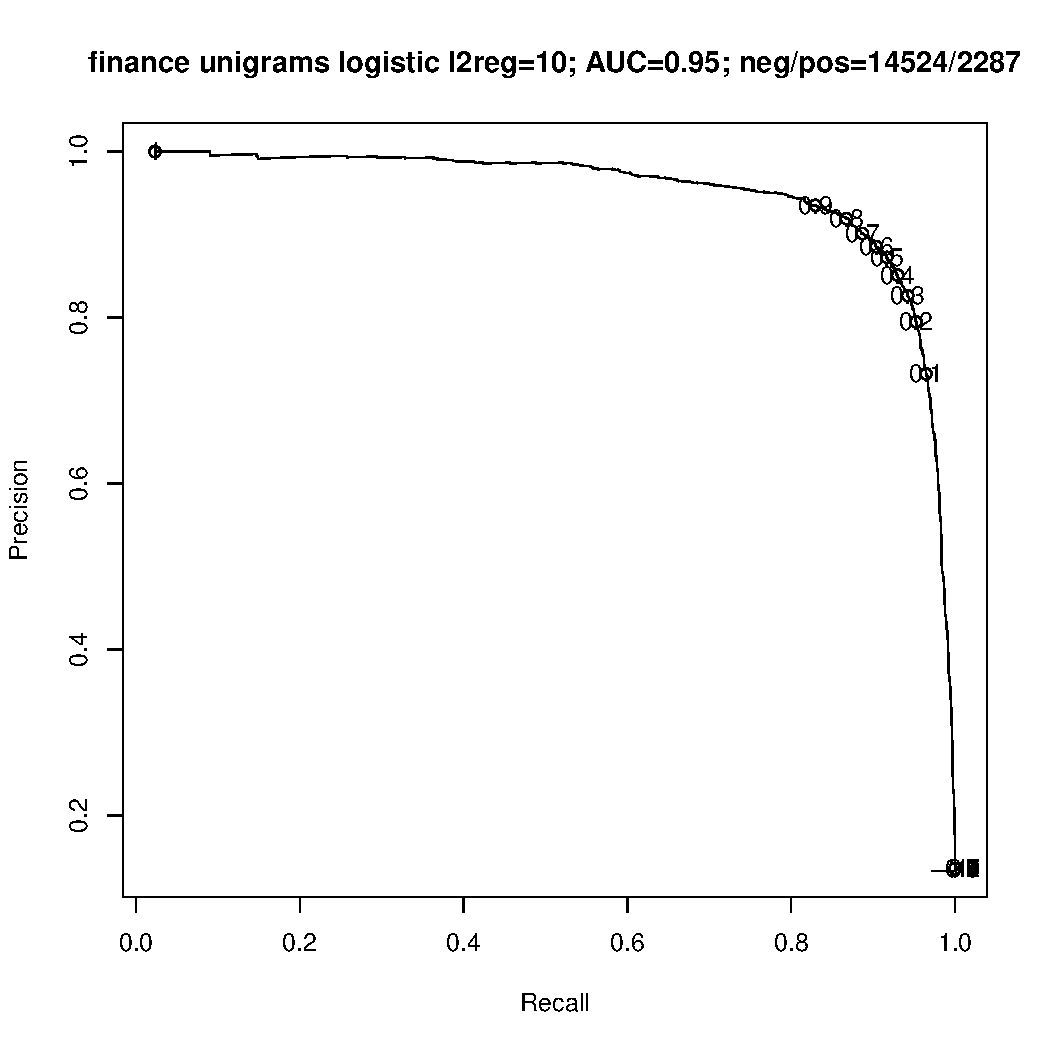
\includegraphics[scale=0.4]{PRcurve_fin.pdf}
\caption{Finance Precision-Recall; unigram logistic , l2reg = 10; AUC = 0.95}\label{PR fin}
\end{figure}

\begin{figure}[H]
\centering
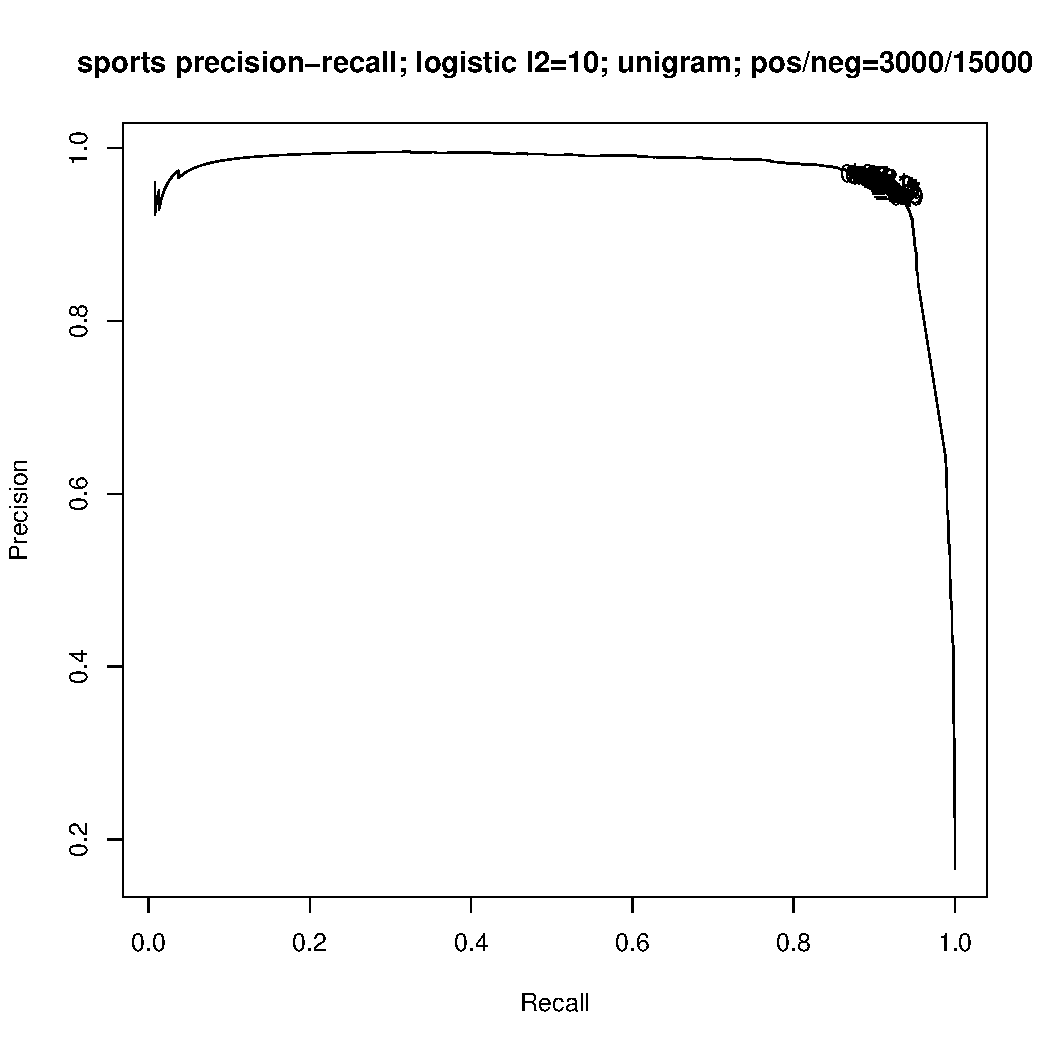
\includegraphics[scale=0.4]{PRcurve_spt.pdf}
\caption{Sports Precision-Recall; unigram logistic , l2reg = 10; AUC = 0.97} \label{PR spt}
\end{figure}

\begin{figure}[H]
\centering
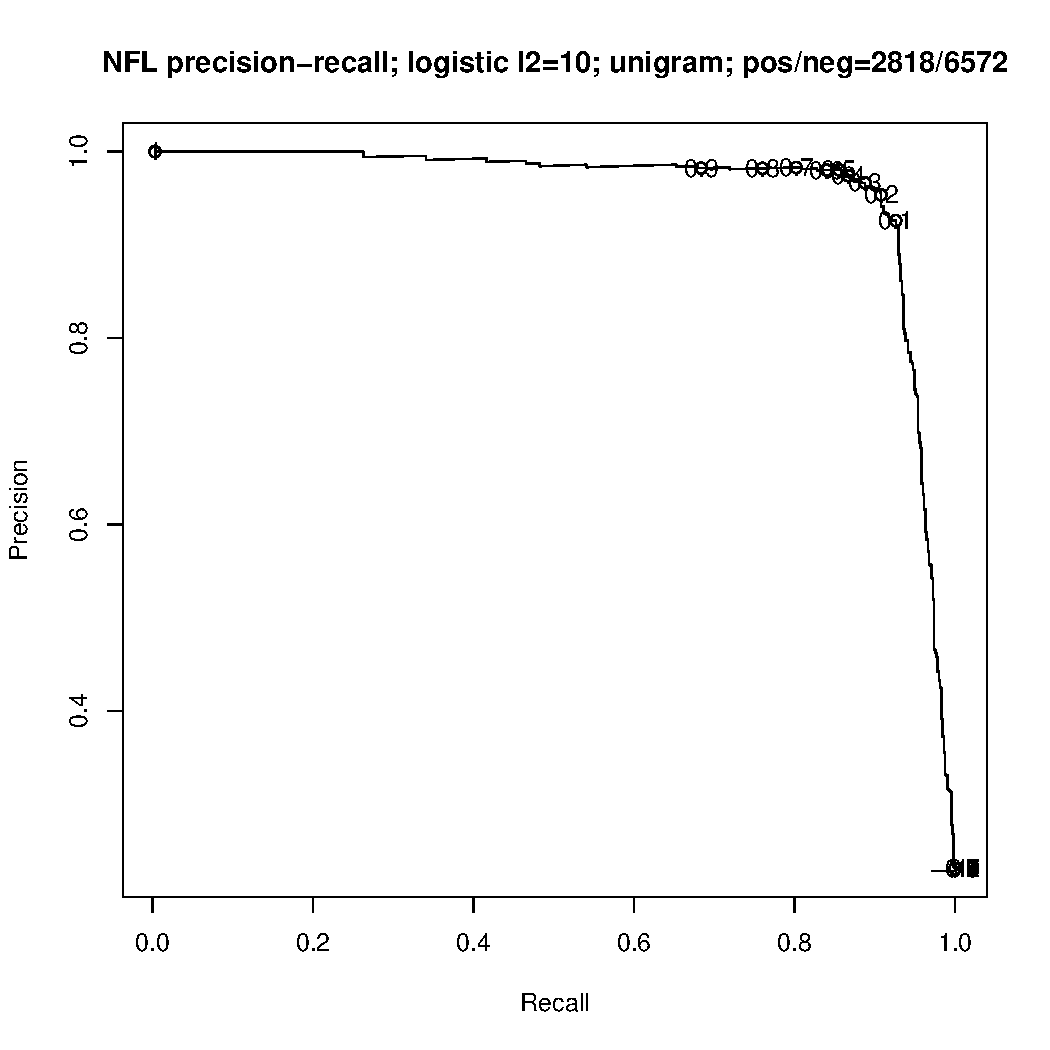
\includegraphics[scale=0.4]{PRcurve_nfl.pdf}
\caption{NFL Precision-Recall; unigram logistic , l2reg = 10; AUC = 0.96}\label{PR nfl}
\end{figure}

Baseline classification error comparison. For the logistic classifier we use threshold at $0$. The data set is always the editorially labeled validation set, since for training and testing data the labels are generated using production filter.

\begin{tabular}{|l|l|l|l|}
\hline
property & labels (+/-) & prod. prec/rec & class. prec/rec \\ \hline
Sports	&  485/394 & 97\%/44\% & 99\%/51\% \\ \hline
Finance & 396/86 & 95\%/35\% & 98\%/50\% \\ \hline
NFL 	& 350/326 & 92\%/59\% & 92\%/89\% \\ \hline
\end{tabular}

So for all three streams, we are able to maintain or improve precision while greatly increase recall rate at a single threshold level. Since the training data is balanced, $0$ threshold makes perfect sense.

Lastly we have the PR curve for the finance stream, using TFIDF classifier (Figure~\ref{PR fin tfidf}).
\begin{figure}[H]
\centering
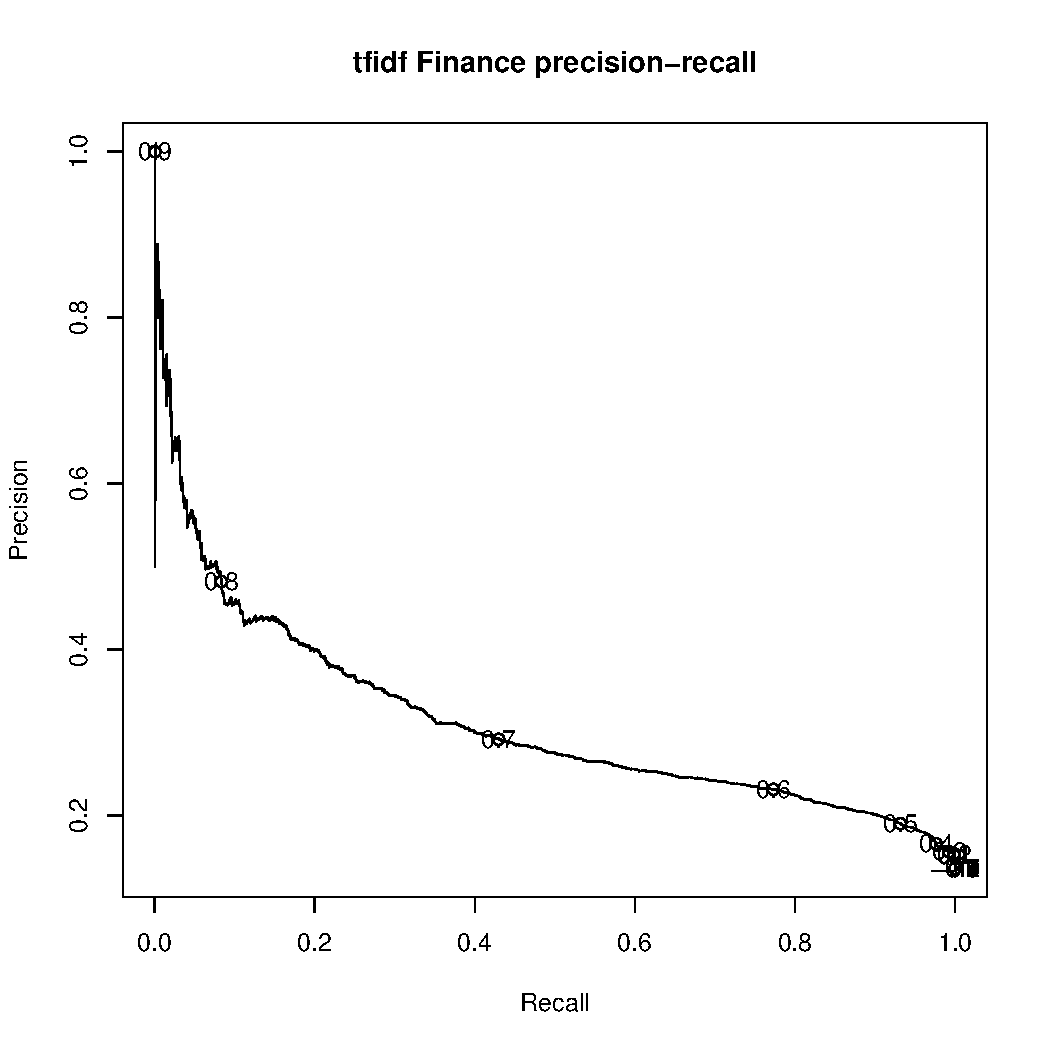
\includegraphics[scale=0.4]{PRcurve_fin_tfidf.pdf}
\caption{Finance Precision-Recall; TFIDF; AUC = 0.31} \label{PR fin tfidf}
\end{figure}

The performance is clearly inferior to logistic classifier.

\subsubsection{Phase 1}
Here we present the ROC AUC for Sports and Finance under four sets of training methodologies:
\begin{enumerate}
\item gmp only: $\rm{score} = \rm{gmp} \times e^{-\beta \Delta T}$;
\item flat dot-product (no SRQ) + gmp: $\rm{score} = (\alpha_0 \rm{gmp} + \alpha_1 \langle \bfu,\bfd\rangle ) e^{-\beta \Delta T}$;
\item SRQ + gmp: $\rm{score} = (\alpha_0 \rm{gmp} + \alpha_1 \langle \bfq \circ \bfu, \bfd \rangle) e^{-\beta \Delta T}$;
\item SRQ with negative pruning + gmp: $\rm{score} = (\alpha_0 \rm{gmp} + \alpha_1 \langle \widetilde{\bfq} \circ \bfu, \bfd \rangle) e^{-\beta \Delta T}$, where $\widetilde{\bfq}_i = 0$ if $\bfq_i \le 0$.
\end{enumerate}

\begin{tabular}{|l|l|l|}
\hline
Method & Sports AUC & Finance AUC\\ \hline
gmp only & 0.58 & 0.62 \\ \hline
flat + gmp & 0.61 & 0.61 \\ \hline
SRQ + gmp & 0.62 & 0.63 \\ \hline
SRQ prune + gmp & 0.64 & 0.65 \\ \hline
\end{tabular}
\subsubsection{phase 2}


\subsubsection{Phase 3}



We illustrate the results in Figure~\ref{DD curve} with a single user session. 
\begin{figure}[H]
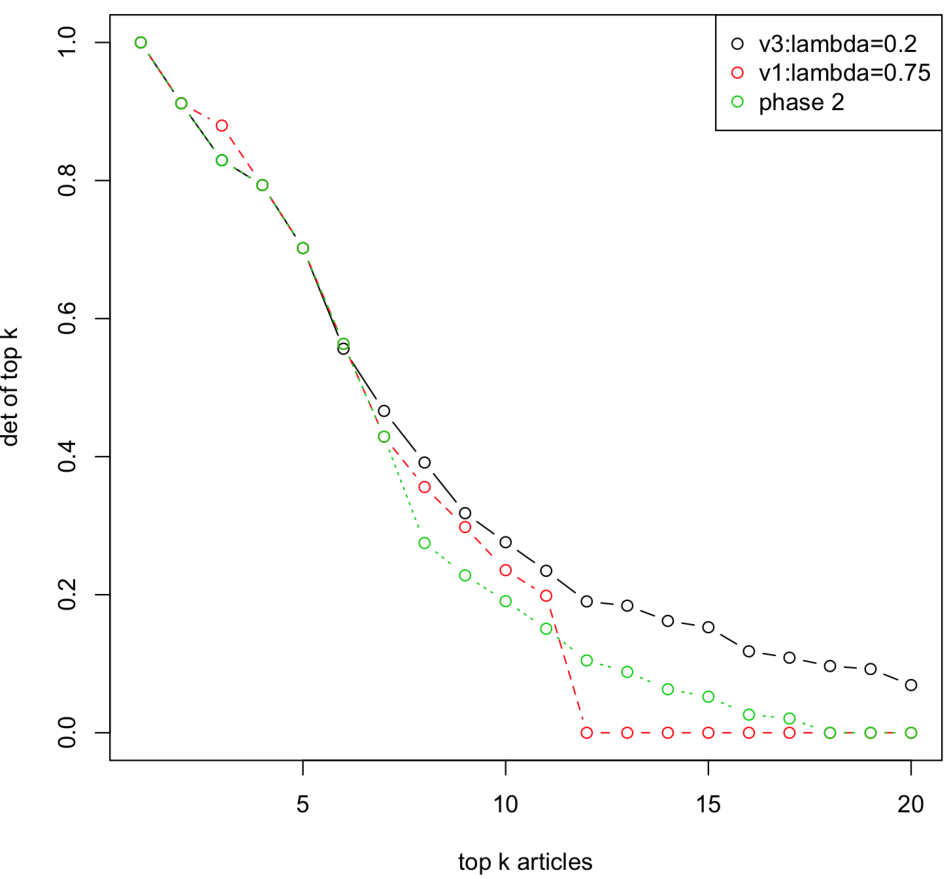
\includegraphics[scale=0.4]{DDcurve.pdf}
\caption{Determinantal Diversity Curve}\label{DD curve}
\end{figure}

\begin{figure}[H]
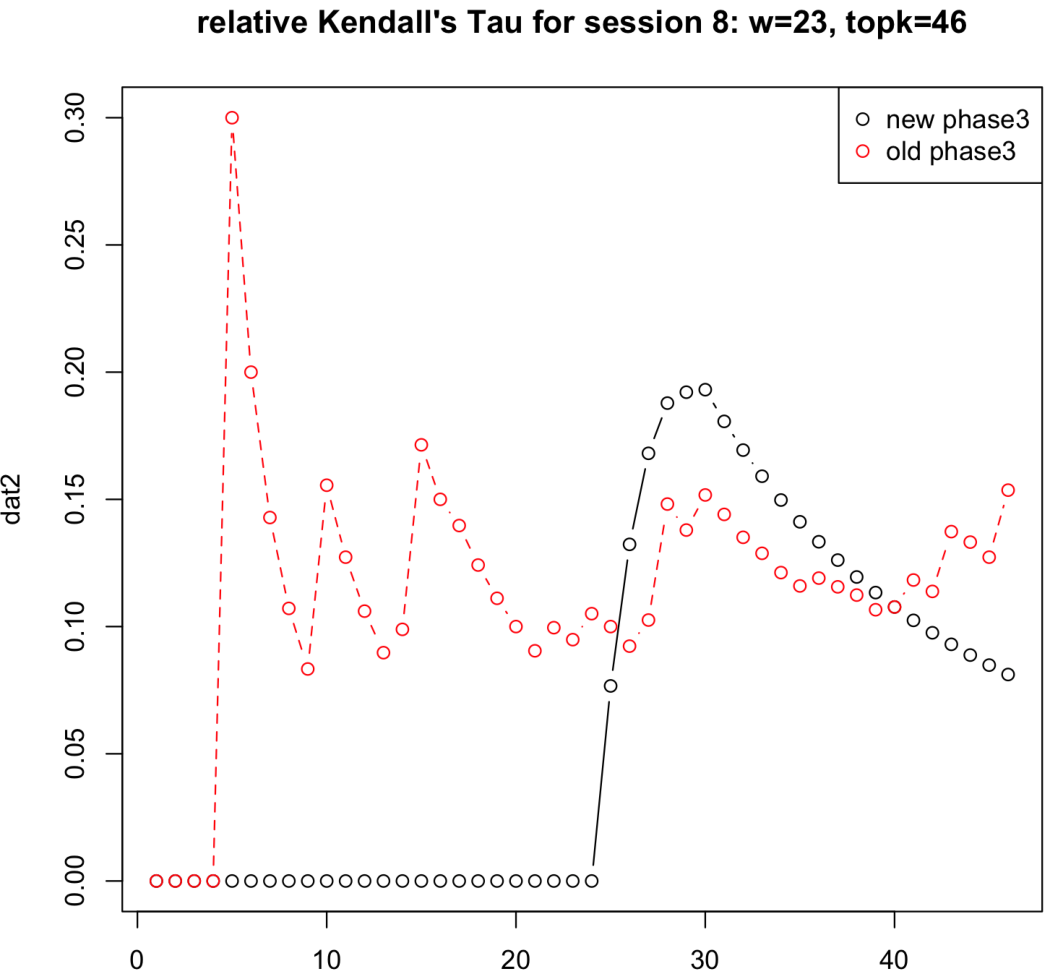
\includegraphics[scale=0.4]{KTcurve.pdf}
\caption{Kendall's Tau Curve}
\end{figure}

In terms of determinantal diversity, algorithm v3 outperforms v1 (so-called MMR approach) or with no diversity at all, consistently across all top k positions, with only one exception at position 3. More importantly, by design v3 preserves the original order from phase 2 ranking up to the end of the first window limit, thus the Kendall's metric is flat at 0 for the duration of the first window. After the first window is exceeded, there is a momentary spike in top k Kendall tau metric, followed by rapid decrease to a level below that of v1. 

\appendix
\section{Diversity Ranking Results} \label{appendix diversity}
Here we present the top 24 articles ranked by both algorithms v1 and v3 for a randomly chosen session on the Finance stream.

Ranking of finance articles according to algorithm v1:
\ssmall{
\begin{verbatim}
ph2    ph3    headline
0       0       Carl Icahn says sellers 'completely misinterpreted' Apple's results"
1       1       Bad Sign for Yahoo: Alibaba's Growth Slows"
2       2       Steady Fed policy could steady markets"
4       3       Indonesia Stocks Rise Most in 2 Weeks on Morgan Stanley Upgrade"
3       4       Electronic Arts Sales Come Up Short in Console Transition"
11      5       NYSE stocks posting largest volume increases"
8       6       Ezcorp 1Q results top views, shares jump"
7       7       VMware Falls 5%: Q1 Rev View In-Line, Year Rev View Beats"
9       8       AT&T swings to 4th-quarter profit of $6.9 billion on higher revenue"
14      9       AT&T reports profit on pension gain"
13      10      Amgen earnings beat forecasts, but 2014 outlook leaves investors cold"
16      11      AT&T revenue rises in fourth quarter"
26      12      Check Point Advances to 12-Year High as Earnings Beat Estimates"
23      13      Seagate Technology Earnings Miss In Difficult Market"
15      14      Stocks End Higher; Data, Earnings in Focus"
28      15      Why Swift Transportation (SWFT) Is Rising Today"
38      16      Dow Today: E.I. Du Pont De Nemours & Company (DD) Lower"
43      17      Remaking star fund managers to fit inside an ETF"
29      18      Builders Rise On D.R. Horton Earnings, Home Prices"
20      19      Stocks Higher In Afternoon; Polaris Trips Sell Rule"
34      20      Rent-A-Center shares fall on disappointing 4Q"
52      21      China Credit Repays Principal to Investors of Bailed-Out Trust"
53      22      Sumitomo Mitsui Quarterly Profit Falls 9.3% on Bond-Trading Drop"
37      23      Chipotle Earnings Seen Heating Up On Expansion Plans"
\end{verbatim}}

Ranking of the same 200 articles according to v3 (lambda = 0.10, w=24):
\ssmall{
\begin{verbatim}
ph2    v3    headlines
0       0       Carl Icahn says sellers 'completely misinterpreted' Apple's results
1       1       Bad Sign for Yahoo: Alibaba's Growth Slows
2       2       Steady Fed policy could steady markets
3       3       Electronic Arts Sales Come Up Short in Console Transition
4       4       Indonesia Stocks Rise Most in 2 Weeks on Morgan Stanley Upgrade
7       5       VMware Falls 5%: Q1 Rev View In-Line, Year Rev View Beats
8       6       Ezcorp 1Q results top views, shares jump
9       7       AT&T swings to 4th-quarter profit of $6.9 billion on higher revenue
10      8       NYSE stocks posting largest volume decreases
13      9       Amgen earnings beat forecasts, but 2014 outlook leaves investors cold
23      10      Seagate Technology Earnings Miss In Difficult Market
26      11      Check Point Advances to 12-Year High as Earnings Beat Estimates
28      12      Why Swift Transportation (SWFT) Is Rising Today
29      13      Builders Rise On D.R. Horton Earnings, Home Prices
34      14      Rent-A-Center shares fall on disappointing 4Q
37      15      Chipotle Earnings Seen Heating Up On Expansion Plans
38      16      Dow Today: E.I. Du Pont De Nemours & Company (DD) Lower
41      17      American Airlines posts $2 billion loss on charges
43      18      Remaking star fund managers to fit inside an ETF
49      19      Maruti Net Income Misses Estimates After Discounts
52      20      China Credit Repays Principal to Investors of Bailed-Out Trust
53      21      Sumitomo Mitsui Quarterly Profit Falls 9.3% on Bond-Trading Drop
54      22      What to expect from Obamacare bellwether Wellpoint
61      23      [video] Why hedging will be key this year
\end{verbatim}}

Version 1 often does not properly eliminate articles with very similar content, judging from their headlines, as  the three almost back-to-back AT\&T articles demonstrate. Equally serious is the observation that many articles under v1 get reversed in their relative order for no apparently good reason. The minimally disruptive nature of v3 makes it an at least locally optimal meta-algorithm on top of phase 2 gbdt ranking.
%
% The following two commands are all you need in the
% initial runs of your .tex file to
% produce the bibliography for the citations in your paper.
\bibliographystyle{abbrv}
\bibliography{gs-ranking.bib}  % sigproc.bib is the name of the Bibliography in this case

\end{document}
